\documentclass{article}
\usepackage[utf8]{ctex}
\usepackage{lineno,hyperref, tablefootnote, booktabs, graphicx,  subfigure, amsmath}
\usepackage[margin=1in]{geometry} %页边距


\usepackage{listings}
\usepackage{xcolor}
\lstset{
%行号
numbers=left,
%背景框
framexleftmargin=10mm,
frame=none,
%背景色
%backgroundcolor=\color[rgb]{1,1,0.76},
backgroundcolor=\color[RGB]{245,245,244},
%样式
keywordstyle=\bf\color{blue},
identifierstyle=\bf,
numberstyle=\color[RGB]{0,192,192},
commentstyle=\it\color[RGB]{0,96,96},
stringstyle=\rmfamily\slshape\color[RGB]{128,0,0},
%显示空格
showstringspaces=false
}

\title{数据库系统概论-项目报告}
\author{张晨 2017011307}

\begin{document}
\maketitle

\section{功能概述}
\subsection{必做功能}
\begin{itemize}
    \item 基于页式文件系统的记录管理
    \item 基于B树的索引管理
    \item 数据库、数据表、键、列的创建、删除、更改
    \item 数据表的增删改查
\end{itemize}
\subsection{选做功能}
\begin{itemize}
    \item 索引的创建、删除
    \item 多表连接查询
    \item 聚集查询,包括AVG,SUM,MAX,MIN
    \item 正则表达式的模式匹配、模糊查询
    \item 利用索引加速
    \item 支持复杂表达式作为更新内容
    \item update支持where子句
    \item Unique索引
    \item B树的常数优化
    \item 使用copy from加载数据库
    \item 表的重命名
\end{itemize}
\section{系统架构设计}
如图\ref{fig:structure}所示。最底层使用了RedBase提供的页式文件系统,记录管理模块访问页式文件系统进行记录的增删改查,索引模块使用记录管理模块作为底层系统,将每个节点视为一条记录(此处与RedBase和本作业架构有区别)。在此基础上建立系统管理模块(负责表结构的维护)和查询解析模块(负责数据的增删改查)。使用Lex/Yacc实现SQL命令的解析,并调用上述两模块。
\begin{figure}[htbp]
    \centering
    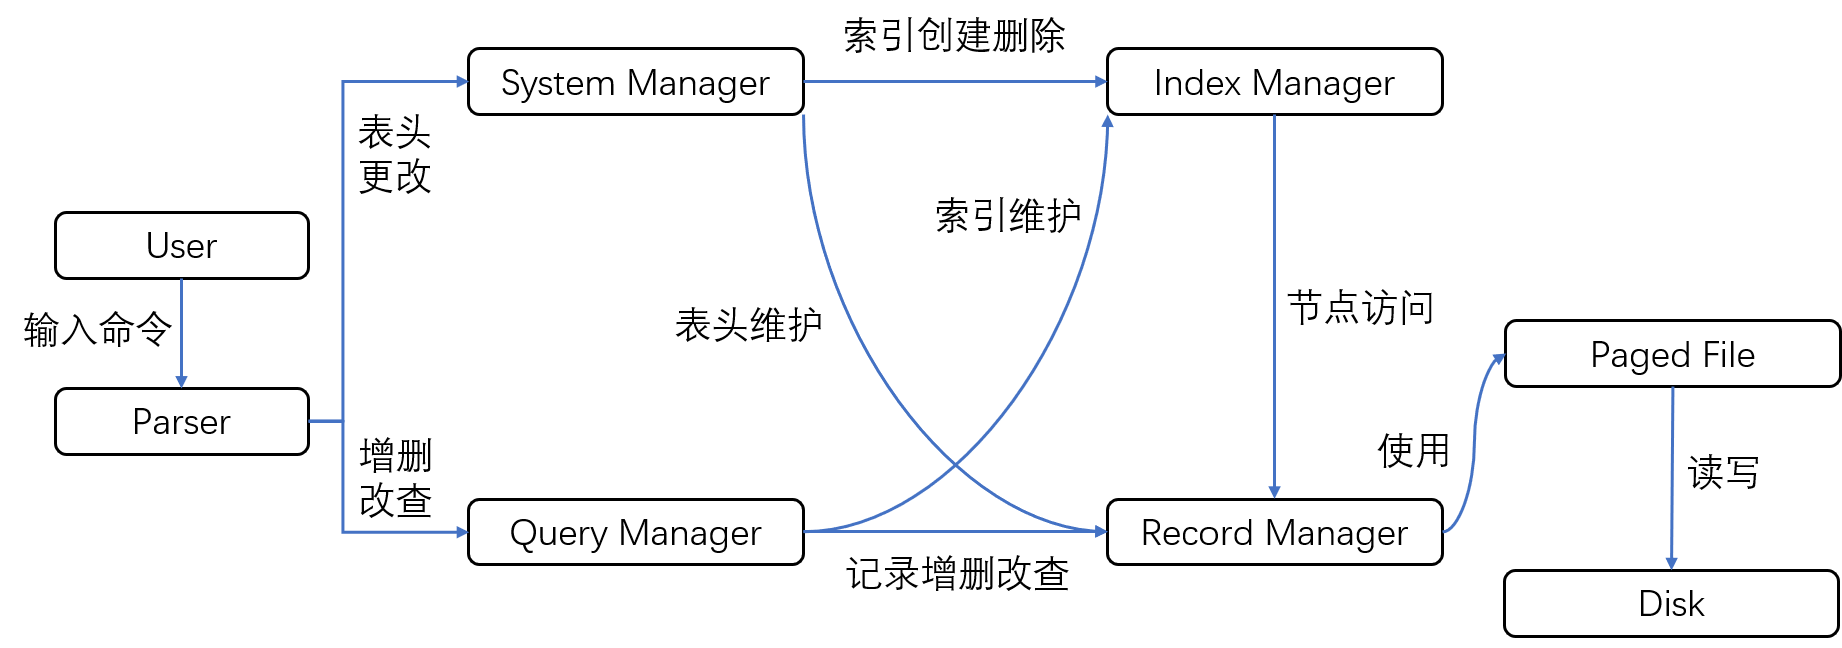
\includegraphics[width=.8\textwidth]{figure/structure.png}
    \caption{数据库的系统架构}
    \label{fig:structure}
\end{figure}
\section{各模块详细设计}
\subsection{记录管理模块}
使用CS346中的页式文件系统与系统设计,实现了新建文件、删除文件、打开文件、关闭文件、插入记录、删除记录、更新记录、获取属性值满足特定条件的记录。

每个记录文件中的记录都是定长的,第一页记录文件中的的记录大小,每页的记录条数,最后一个页的编号,调用方的元数据大小,剩余空间暴露给调用方以储存对该记录文件的描述(如数据表的表头信息等)。每一页最前面使用一个01串表示对应位置是否存在记录。

\subsection{索引模块}
基于B树实现了新建索引,删除索引,打开索引,关闭索引,插入节点,删除节点,获取属性值满足特定条件的节点。使用B树而非B+树的原因是,在CS346的架构中,数据的值允许重复,因而需要将RID也当做树排序的关键字,更详细的分析见附录。

每条索引记录其对应的RID及各个变量的值(的二进制表示),为了保证字符串不会被截断,还存了每个值的长度。
B树的每个节点记录父亲的存储位置,自己的存储位置,本节点包括的索引记录,孩子们的存储位置,孩子的数量。
在元数据中,记录索引的各个变量的类型、最大长度,B树每层的最大节点数,树根的位置。

B树更新、查询的过程中,与文件系统的交互被抽象成了insert, delete, get, update四种操作。文件系统直接使用来了记录管理模块,将每个B树节点视为一条记录。实现了B树的上溢修复和下溢修复。

扫描仅需从根开始按照一定规则对B树进行遍历。实现了等于、不等于、大于、大于等于、小于、小于等于共计六种操作。不等于的合法解至多为2段连续区间,其余都至多为1段连续区间。因而,还通过树的结构推断出某些树中节点所存的袁术一定是/不是合法解,从而进行剪枝及降低比较次数。

\subsection{系统管理模块}
实现了数据库的创建、删除、切换,表的创建删除,主键、外键、unique键的添加删除,列的添加删除,索引的添加删除。在操作前都进行了大量合法性检查,以保证数据库的完整性约束。
\subsubsection{文件系统}
一个数据库对应一个同名的文件夹,新建、删除数据库对应于新建、删除文件夹,切换数据库时将程序的“当前目录”切换到该文件夹。

一个表对应于数据库文件夹中的一个同名文件,在记录管理模块的元数据中存放表头信息,表头信息包括表名、各变量信息、主键、外键、unique key、被链接到自己主键的其他表外键、创建的索引。每条数据被视为一条记录。每个索引对应数据库文件夹中以表名为前缀的一个文件,文件中保存相应的索引记录。

\subsubsection{具体实现}

对于数据库的创建、删除、切换操作直接调用相应的系统函数,调用前会先查看相应的文件夹是否存在。在系统管理模块中也记录了当前切换到的数据库名。

表的信息查询会获取当前文件夹中的文件名,由文件名分析出创建的所有表。

表的建立、删除会访问记录管理模块,通过记录管理模块的报错保证表名的唯一性和删除的正确性。在表的建立前,也会检查表头信息的合理性。

表头的更新及键的更新会依次在系统管理和查询解析模块中询问操作的合法性,只有校验了操作完全合法才会执行。校验的内容包括是否切换到一个数据库中、相应的名字是否存在、类型是否匹配、是否创建了多个主键、是否会破坏完整性约束等等。完整性约束在查询解析模块中检查,包括主键及unique key是否非空且无冲突、外键是否都有对应值等等。

因为在添加及更新时,会频繁地查询唯一性约束,故自动为主键及unique key建立索引,以减少校验及查询的时间。

\subsection{查询解析模块}
实现了增删改查,SELECT支持多表连接、聚集查询,SET支持四则运算,WHERE子句支持常见条件表达式、NULL的判断、整数和字符串比较、正则匹配。在对数据库进行操作前都先进行检查,主要包括命名检查、类型检查、约束检查等。
\subsubsection{增删改查的实现}
Insert,对类型、主键、外键、unique等进行检查后直接添加。

Delete,进行校验后,使用select选出所有要删的记录,进行删除。

Update,选出要更改的记录,检查更改后是否仍然满足唯一性约束,进行更改。检查唯一性约束的方法是,所有要修改的记录是没有重复的,且它们和未修改的记录之间没有重复。

Select,首先使用每个表单独的选择条件选出内容,再将它们进行连接。最后执行聚集查询。
\subsubsection{复杂命令的支持}
Set支持复杂的表达式,表达式中可出现列名、常数、四则运算、括号。在命令解析阶段,即对表达式建立抽象语法树。之后解析抽象语法树的各个节点,将其对应到一个数或一个(表名,列号)的二元组。计算时,直接利用树结构自底向上计算。

\subsubsection{多表连接查询算法}
首先用每个表单独的约束在每个表中做筛选,之后按选出的条数从小到大依次连接。连接操作使用STL的MAP降低复杂度。


\subsection{命令解析模块}
基于Lex/Yacc实现了SQL命令的解析及抽象语法树的构建。在抽象语法树的最高层,进行命令的执行。

\subsection{单元测试}
分别对记录管理模块、索引模块编写了单元测试程序,若单元测试失败,会 assert 退出或返回 Error Code。

系统管理模块及查询解析模块则直接使用SQL语句进行测试。

\section{主要接口说明}
\subsection{记录管理模块}
\subsubsection{Record}
一个Record类表示一条记录,可以获取其值,设置其值,获取其存储位置。
\begin{lstlisting}[language=C++]
RC GetData(char * &pData);
RC MoveData(char* &pData);
RC GetRid (RID &rid); 
void SetValue(const char* _data, int _len, RID _rid);
void CopyTo(RM_Record& rec);
\end{lstlisting}
\subsubsection{FileHandle}
一个FileHandle对应一个文件,可以通过与页式文件系统的交互,对记录进行增删改,进行记录的简单遍历,获取、更新元数据信息。
\begin{lstlisting}[language=C++]
RC GetRec     (const RID &rid, RM_Record &rec) const;
RC InsertRec  (const char *pData, RID &rid);
RC DeleteRec  (const RID &rid);
RC UpdateRec  (const RM_Record &rec);

RC GetMetaSize(int& size);
RC GetMeta(char* pData, int& size);
RC SetMeta(const char* pData, int size);

RC ForcePages (PageNum pageNum = ALL_PAGES);

RC GetFirstRec(PageNum& pageNum, SlotNum& slotNum,  RM_Record &rec) const;
RC GetNextRec(PageNum& pageNum, SlotNum& slotNum,  RM_Record &rec) const;
\end{lstlisting}
\subsubsection{FileScan}
FileScan用于对文件进行遍历。
\begin{lstlisting}[language=C++]
RC OpenScan  (const RM_FileHandle &fileHandle);
RC GetNextRec(RM_Record &rec);
RC CloseScan ();
\end{lstlisting}
\subsubsection{Manager}
Manager用于文件的创建、删除、打开、关闭,实现为单例。
\begin{lstlisting}[language=C++]
RC CreateFile (const std::string& fileName, int recordSize,
    char* pMeta = nullptr, int metaSize = 0);
RC DestroyFile(const std::string& fileName);
RC OpenFile   (const std::string& fileName, RM_FileHandle &fileHandle);
RC CloseFile  (RM_FileHandle &fileHandle);
\end{lstlisting}
\subsection{索引管理模块}
\subsubsection{IndexHandle}
用于B树和记录管理的交互,对B树,有插入、删除操作。对记录管理,可新建、更新、删除等。
\begin{lstlisting}[language=C++]
RC InsertEntry     (const std::vector<std::string> &pData, const RID &rid);
RC DeleteEntry     (const std::vector<std::string> &pData, const RID &rid);
RC ForcePages      ();

IX_BTNode get(RID pos);
IX_BTNode loadRoot();
void setRoot(const RID& pos);
void update(IX_BTNode& node);
RID newNode(IX_BTNode& tr);
void deleteNode(IX_BTNode& tr);
\end{lstlisting}
\subsubsection{IndexScan}
用于对索引进行扫描,返回符合条件的结果。条件包括大于、大于等于、小于、小于等于、等于、不等于六种运算符。
\begin{lstlisting}[language=C++]
RC OpenScan      (IX_IndexHandle &indexHandle,
				  CompOp      compOp,
				  const std::vector<std::string> &value,
				  ClientHint  pinHint = NO_HINT);       
RC GetNextEntry  (RID &rid);
RC CloseScan     ();
\end{lstlisting}
\subsubsection{Manager}
用于索引的新建、删除、打开、关闭。实现为单例。
\begin{lstlisting}[language=C++]
RC CreateIndex(const char *fileName, int indexNo,
			   const std::vector<AttrType> &attrType,
			   const std::vector<int> &attrLength);
RC DestroyIndex(const char *fileName, int indexNo);
RC OpenIndex(const char *fileName, int indexNo,
             IX_IndexHandle &indexHandle);
RC CloseIndex(IX_IndexHandle &indexHandle);
\end{lstlisting}

\subsection{系统管理模块}
\subsubsection{Manager}
对数据库系统进行管理的类,实现了系统管理模块的各个接口,以下是其对外接口。
\begin{lstlisting}[language=C++]
RC UseDb      (const std::string& dbName);    // Use the database
RC CreateDb   (const std::string& dbName);    // Create the database
RC DropDb     (const std::string& dbName);    // Drop the database
RC ShowAllDb  ();

RC CreateTable(const std::string& relName, const TableInfo& table);
RC DropTable(const std::string& relName);
RC ShowTable(const std::string& relName);
RC ShowTables();

RC CheckAddPrimaryKey(const std::string& tbName,
                      const std::vector<std::string>& attrNames);
RC AddPrimaryKey(const std::string& tbName,
                 const std::vector<std::string>& attrNames);
RC DropPrimaryKey(const std::string& tbName);

RC AddForeignKey(const std::string& tbName, const ForeignKeyInfo& fKey);
RC DropForeignKey(const std::string& tbName, const std::string& fkName);

RC CheckAddUniqueKey(const std::string& tbName, const std::string& pkName,
                     const std::vector<std::string>& pKeys);
RC AddUniqueKey(const std::string& tbName, const std::string& pkName,
                const std::vector<std::string>& pKeys);
RC DropUniqueKey(const std::string& tbName, const std::string& pkName);

RC AddAttr(const std::string& tbName, const AttrInfo& attr);
RC DropAttr(const std::string& tbName, const std::string& attrName);
RC ChangeAttr(const std::string& tbName, const std::string& attrName,
              const AttrInfo& newAttr);

RC CheckCreateIndex(const std::string& tbName, const std::string& idxName,
                    const std::vector<std::string>& attrNames);
RC CreateIndex(const std::string& tbName, const std::string& idxName,
               const std::vector<std::string>& attrNames);
RC DropIndex(const std::string& tbName, const std::string& idxName);


RC GetTable(const std::string& relName, TableInfo& table);
RC UpdateTable(const std::string& tbName, const TableInfo& table);
RC ShuffleForeign(const std::string& srcTbName, ForeignKeyInfo &key,
                  const std::vector<std::string>& refAttrs);
RC ShuffleForeign(const TableInfo& srcTable, ForeignKeyInfo &key,
                  const std::vector<std::string>& refAttrs);
RC LinkForeign(const std::string& reqTb, const ForeignKeyInfo &key);
RC DropForeignLink(const std::string& refTb, const std::string& fkName);
\end{lstlisting}
\subsection{查询解析模块}
\subsubsection{Manager}
对数据库进行增删改查的类,以下是其对外接口。
\begin{lstlisting}[language=C++]
RC Insert(const std::string& tbName,
          const std::vector<std::string>& rawValues);
RC Delete(const std::string& tbName,
          const std::vector<RawSingleWhere>& rawConds);
RC Update(const std::string& tbName,
          const std::vector<RawSetJob> &rawJobs,
          const std::vector<RawSingleWhere>& rawConds);
RC Select(const std::vector<std::string>& tbNames,
                std::vector<RawTbAttr>& rawSelectors, 
          const std::vector<RawSingleWhere>& singleConds,
          const std::vector<RawDualWhere>& rawDualConds,
                GatherOp gOp);
RC Desc(const std::string& tbName);

bool CanAddPrimaryKey(const std::string& tbName,
                      const std::vector<std::string>& attrNames);
bool CanAddForeignKey(const std::string& tbName,
                      const ForeignKeyInfo& fKey);
bool CanChangeCol(const std::string& tbName);
bool CanCreateIndex(const std::string& tbName,
                    const std::vector<std::string>& attrNames);
bool CanAddUniqueKey(const std::string& tbName,
                     const std::vector<std::string>& attrNames);

RC AddPrimaryKey(const std::string& tbName);
RC AddUniqueKey(const std::string& tbName, const std::string& pkName);
RC InitIndex(const std::string& tbName,
             const std::string& idxName);
\end{lstlisting}
\section{实验结果}
通过了助教的37条测例中的34条,未通过的包括Group by,嵌套查询,级联更新删除。另外通过了对于复杂表达式的检查。

\section{小组分工}
单人完成

\section{参考资料}
\begin{itemize}
    \item 《数据库大作业详细说明》
    \item RedBase Project \url{https://web.stanford.edu/class/cs346/2015/redbase.html}
    \item 《数据结构》 邓俊辉
\end{itemize}
\appendix
\section{附录:选用B树的原因}
在RedBase及本作业的说明中,都要求使用B+树存储属性值到RID的映射。但我认为这里使用B树更为合适。在我的理解中,B+树相比B树主要有以下几点优点:
\begin{enumerate}
    \item 所有数据均存储在叶子结点,因此内部节点可以存更少的东西,以增加分叉数,降低树高,从而减少IO次数。
    \item 叶子节点通过双向链表连接,使得遍历更加方便。
\end{enumerate}

但是,在CS346中,是允许属性值重复的,需要在树中维护同一属性值的所有RID。如果采用B+树实现,在内部节点中不应存属性值的RID,否则B+树的第一条优势将不复存在。经过思考及与同学的讨论,我得出了以下两种可行的实现方式,但是它们都存在自己的问题。

\begin{enumerate}
    \item 使用属性+RID作为B+树排序的key,但在内部节点仅存属性值,不存RID。每次插入/删除时,通过全局二分节点在树中的排名找到相应的节点。很明显,这种实现方法最大的问题在于多了二分的一个log的复杂度。
    \item 仅使用属性作为B+树排序的key。每个叶子结点再使用一个B+树存所有的RID。这种方式首先会大大增加工程难度,其次在性能上也并不优秀。对于重复较多的key,叶子结点中的B+树的深度较大,因而进行访问的时间又较长。但是,重复较多的key一般又正是访问次数较多的key,这使得这种实现方式在理论性能上劣于全局平衡的B+树。
\end{enumerate}

然而,每个节点所需要存的数据仅仅是一个RID,占用的空间不大,因而中间节点省去它并不会明显降低中间节点的存储量。

此外,我认为叶子节点通过双向链表连接,最大的意义是方便工程的实现。但是,使用链表意味着需要对每个数据进行比对,而放弃了树本身能提供的结构信息。如果使用B树实现,对于等于、不等于、大于(等于)、小于(等于)这类基础操作,需要的比较次数会大大降低。

综上所述,我选择B树进行索引。
\end{document}
